\documentclass[10pt,letterpaper]{article}
\usepackage[utf8]{inputenc}
\usepackage[spanish]{babel}
\usepackage{amsmath}
\usepackage{amsfonts}
\usepackage{amssymb}
 \usepackage{float}
\usepackage{graphicx}
\usepackage{subfiles}
\usepackage{enumitem}
\usepackage[affil-it]{authblk}
\usepackage{array}
\usepackage{tabularx}
\usepackage{multicol}
\usepackage{slashbox}
\usepackage{diagbox}
\usepackage{slashbox,multirow}
\usepackage{enumitem}
\usepackage{mathtools}
\usepackage{pstricks}
\usepackage{pgfplots}
\usepackage{enumitem}
\usepackage{tikz}
\usepackage{calc}
\usepackage{ifthen}
\usepackage{mathrsfs} %Contiene el Signo de Transformada de Laplace
\usepackage{empheq}
\usepackage{svg}
\usepackage[left=2cm,right=2cm,top=2cm,bottom=2cm]{geometry}
\author{Leonardo H. Añez Vladimirovna \footnote{Para cualquier cambio, observación y/o sugerencia pueden enviarme un mensaje al siguiente correo: \texttt{toborochi98@outlook.com}}}
\title{Fórmulas Investigación Operativa II \texttt{(MAT419)}\footnote{Esta es una recopilación de las formulas utilizadas en la materia, sin teoría.}\\{\normalsize Facultad de Ingeniería en Ciencias de la Computación y Telecomunicaciones}\\ \vspace{-0.025cm}\normalsize Universidad Autónoma Gabriel René Moreno}
 \pgfplotsset{compat=1.16}
\begin{document}
\maketitle
\section{Inventarios}
\noindent
\begin{minipage}[t]{.2\textwidth}
\raggedright
Costo Unitario
$$C_1 = \left[\dfrac{\$}{u}\right]$$
\end{minipage}% <---------------- Note the use of "%"
\begin{minipage}[t]{.2\textwidth}
\raggedright
Costo de Hacer el Pedido
$$C_2 = \left[\$ \right]$$
\end{minipage}%
\begin{minipage}[t]{.2\textwidth}
\raggedright
Costo de Hacer el Pedido
$$C_3 = \left[\dfrac{\$}{u\cdot \text{año}}\right]$$
\end{minipage}%
\begin{minipage}[t]{.4\textwidth}
\raggedright
\begin{itemize}
\item $D=$ Demanda  [$\frac{u}{\text{año}}$]
\item $P=$ Producción [$\frac{u}{\text{año}}$]
\item $A=$ Acumulación
\item $L=$ Tiempo Reposición
\end{itemize}
\end{minipage}
\subsection{Cantidad Económica del Pedido (EOQ)}
\begin{itemize}
\item Conocemos la Demanda Anual. $D = \left[ \frac{u}{\text{año}}\right] $
\item Se conoce el tiempo de entrega de pedidos. $L=[\text{días}]$
\item Se conoce $C_1,C_2,C_3$.
\end{itemize}
\begin{enumerate}
\noindent
\begin{minipage}[t]{.33\textwidth}
\raggedright
\item Cant. Económica del Pedido \noindent
$$Q_0 = \sqrt{ \dfrac{2\cdot D \cdot C_2}{C_3}}=[u]$$
\end{minipage}% <---------------- Note the use of "%"
\begin{minipage}[t]{.33\textwidth}
\raggedright
\item Punto de Reposición \noindent
$$R=D'\cdot L = [u]$$
\end{minipage}%
\begin{minipage}[t]{.33\textwidth}
\raggedright
\item Tiempo entre Pedidos \noindent
$$t=\dfrac{1}{N}=\dfrac{Q_0}{D}=[\text{años}]$$
\end{minipage}
\\${ }$\\
\noindent
\begin{minipage}[t]{.5\textwidth}
\raggedright
\item Nro. Pedidos
$$N = \dfrac{D}{Q_0}$$
\end{minipage}% <---------------- Note the use of "%"
\begin{minipage}[t]{.5\textwidth}
\raggedright
\item Ec. del Gráfico de Existencia
$$Q=at+b = -\dfrac{D}{364}+Q_0$$
\end{minipage}%
\item Costos Anuales Óptimos
$$C_T = C_1 D + C_2 \left( \dfrac{D}{Q_0} \right) + C_3 \left( \dfrac{Q_0}{2} \right)$$
\end{enumerate}
\subsubsection*{Donde}
\begin{itemize}
\item $C_1 D$: Costo Anual de Producción
\item $C_2 \left( \dfrac{D}{Q_0} \right)$: Costo Anual de Pedidos
\item $C_3 \left( \dfrac{Q_0}{2} \right)$: Costo Anual de Mantener el Inventario
\end{itemize}
\vspace{0.1cm}
\begin{figure}[H]
\centering
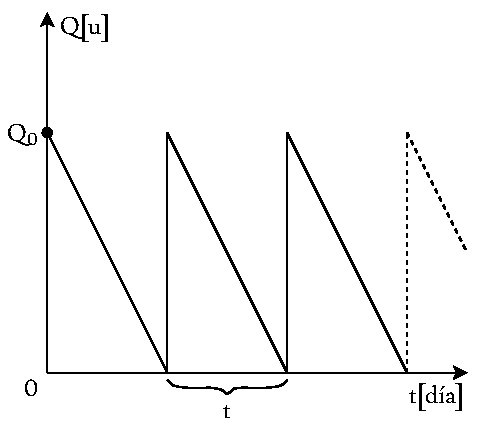
\includegraphics[scale=0.8]{EOQ.pdf}
\end{figure}
\subsection{Clasificación ABC de Inventarios}
\noindent
\begin{minipage}[t]{.5\textwidth}
\raggedright
\begin{align*}
\text{Grupo}=
\begin{cases}
A \rightarrow \text{Artículos de Mayor Precio} \\
B \rightarrow \text{Artículos de Precio Medio} \\
C \rightarrow \text{Artículos Baratos}
\end{cases}
\end{align*}
\end{minipage}% <---------------- Note the use of "%"
\begin{minipage}[t]{.5\textwidth}
\raggedright
$$
\text{Costo Anual}[\$] = \text{Demanda Anual}[u]\cdot \text{Costo Unitario}\left[ \frac{\$}{u}\right]
$$
\end{minipage}
\begin{figure}[H]
\centering
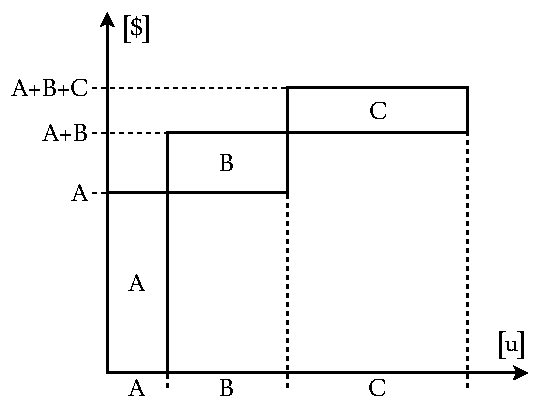
\includegraphics[scale=0.8]{ABC.pdf}
\end{figure}
\subsection{Modelo de Producción de Inventarios}
\begin{itemize}
\item Si o sí producen por tantas.
\item Se produce y vende lo del inventario.
\item Se conoce $P$ y $D$.
\item Se conocen $C_1,C_2,C_3$.
\item Son los procesos discontínuos.
\end{itemize}
\begin{align*}
\boxed{P > D} &\hspace{0.1cm} & \boxed{A=P-D} & \hspace{0.1cm} & P=D (\text{No hay acumulación)}
\end{align*}

\begin{enumerate}
\noindent
\begin{minipage}[t]{.33\textwidth}
\raggedright
\item Cant. Económica del \\ Lote de Producción
$$
Q_0 = \sqrt{\dfrac{2\cdot D C_2}{C_3 \left( 1-\dfrac{D}{P} \right)}} =[u]
$$
\end{minipage}% <---------------- Note the use of "%"
\begin{minipage}[t]{.33\textwidth}
\raggedright
\item Tiempo de producción \\ (Una tanda)
$$
t_1 = \dfrac{Q_0}{P}
$$
\end{minipage}%
\begin{minipage}[t]{.33\textwidth}
\raggedright
\item Tiempo entre \\ Tandas \\
$$
t=\dfrac{Q_0}{D}
$$
\end{minipage}
\\${ }$\\
\noindent
\begin{minipage}[t]{.33\textwidth}
\raggedright
\item Tiempo sin producción \\ (Solo Demanda)
$$
t_2 = t-t_1 = \dfrac{Q_0}{D}-\dfrac{Q_0}{P}
$$
\end{minipage}% <---------------- Note the use of "%"
\begin{minipage}[t]{.33\textwidth}
\raggedright
\item Inventario \\Máximo
$$
I_{max}=A\cdot t_1 = (P-D)\left(\dfrac{Q_0}{P} \right)
$$
\end{minipage}%
\begin{minipage}[t]{.33\textwidth}
\raggedright
\item Numero de Tandas \\ (Pedidos)
$$
N=\dfrac{1}{t} = \dfrac{D}{Q_0}
$$
\end{minipage}
\item Costo Anual de Inventario
$$
C_T = C_1\cdot D + C_2 \left( \dfrac{D}{Q_0} \right) + C_3 \left(\dfrac{Q_0}{2} \right)  \left( 1- \dfrac{D}{P} \right)
$$
\end{enumerate}
\begin{figure}[H]
\centering
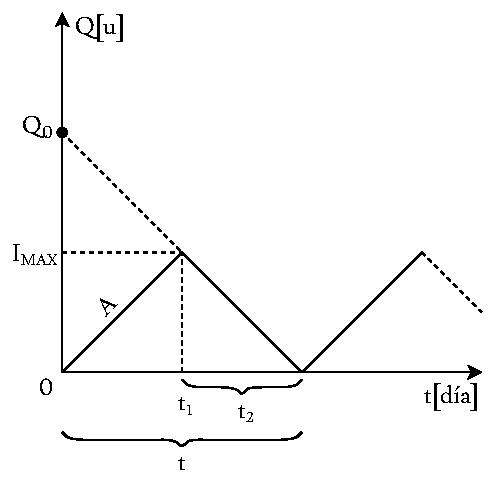
\includegraphics[scale=0.8]{PROD.pdf}
\end{figure}
\subsection{Modelo Probabilístico}
\begin{itemize}
\item $\mu = [\frac{u}{\text{año}}]$
\item $\sigma = [\frac{u}{\text{año}}]$
\item Se conoce $C_1,C_2,C_3$
\item Se conoce $L$ (Tiempo de Reposición)
\item Se determina $\alpha$ (grado de confianza)
\end{itemize}
\begin{enumerate}
\noindent
\begin{minipage}[t]{.25\textwidth}
\raggedright
\item Cantidad Optima \\ del Pedido
$$
Q_0 = \sqrt{\dfrac{2 \cdot  \mu  \cdot  C_2}{C_3}}
$$
\end{minipage}% <---------------- Note the use of "%"
\begin{minipage}[t]{.25\textwidth}
\raggedright
\item Punto \\ de Reposición
$$
R = D' L
$$
\end{minipage}% <---------------- Note the use of "%"
\begin{minipage}[t]{.25\textwidth}
\raggedright
\item Número de\\ Pedidos
$$
N=\dfrac{\mu}{Q_0}
$$
\end{minipage}% <---------------- Note the use of "%"
\begin{minipage}[t]{.25\textwidth}
\raggedright
\item Existencia de\\ Seguridad
$$
S = z \cdot \sigma_L
$$
\end{minipage}
\\${ }$\\
\begin{minipage}[t]{.33\textwidth}
\raggedright
\item Sigma
$$
\sigma_L = \sigma \cdot \sqrt{L}
$$
\end{minipage}%
\begin{minipage}[t]{.33\textwidth}
\raggedright
\item Punto de Reposición \\ (Con colchon de seguridad)
$$
R'=R+S
$$
\end{minipage}%
\begin{minipage}[t]{.33\textwidth}
\raggedright
\item Calculo de $z$ (si es necesario interpolar)
$$
z = \epsilon + \Delta z
$$
\end{minipage}
\item Costos Anuales
$$
C_T = C_1 \cdot\mu + C_2 \left( \dfrac{\mu}{Q_0}\right) + C_3 \left( \dfrac{Q_0}{2}+S \right)
$$
\end{enumerate}
\subsubsection*{Donde}
\begin{itemize}
\item $z=$ Desviación Normalizada
\item $\sigma_L=$ Desviación Estandar por tiempo guía
\end{itemize}
\begin{figure}[H]
\centering
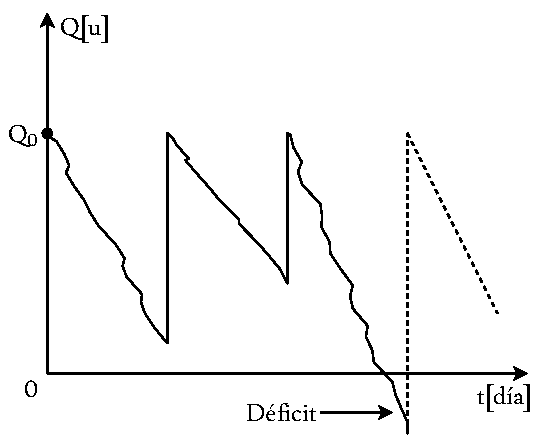
\includegraphics[scale=0.8]{PROB.pdf}
\end{figure}
\section{Decisiones}
\subsection{Riesgo}
\begin{minipage}[t]{.5\textwidth}
\raggedright
\begin{itemize}
\item VME (Valor Monetario Esperado)
\item COE (Costo de Operacion Esperado)
\item VEIP (Valor Esperado de Informacion Perfecta)
\end{itemize}
\end{minipage}%
\begin{minipage}[t]{.5\textwidth}
\raggedright
\vspace{-0.8cm}
\begin{align*}
& \text{VEIP} = \text{COE} \\
& \text{VEIP} = \text{VECC} - Max_{VME}
\end{align*}
\end{minipage}%
\subsection{Incertidumbre}
\begin{itemize}
\item Laplace: $P(S_n)$
\item Wald (Pesimista): Mejor de los Peores Resultados
\item Hurwicz: $Max_{columna}\cdot \alpha + Min_{columna}\cdot (1-\alpha)$. ($\alpha$ indice de optimismo)
\item Maximax: Máximo de máximos.
\item SAVAGE $\approx$ COE
\end{itemize}
\section{Colas}
\begin{itemize}
\item Llegadas aleatorias, distribución tipo Poisson.
\item Tasa de servicio aleatoria
\item $\mu \geq \lambda$\footnote{Si $\lambda\geq\mu$ la cola crece al infinito.}
\end{itemize}
\begin{enumerate}

\begin{minipage}[t]{.25\textwidth}
\raggedright
\item Tiempo en Sistema
$$
W_s = \dfrac{1}{\mu - \lambda}
$$
\end{minipage}%
\begin{minipage}[t]{.25\textwidth}
\raggedright
\item Tiempo en Cola
$$
W_q = \dfrac{\lambda}{\mu\cdot (\mu - \lambda)}
$$
\end{minipage}%
\begin{minipage}[t]{.25\textwidth}
\raggedright
\item Clientes en Sistema
$$
L_s = \dfrac{\lambda}{\mu - \lambda}
$$
\end{minipage}%
\begin{minipage}[t]{.25\textwidth}
\raggedright
\item Clientes en Cola
$$
L_q = \dfrac{\lambda^2}{\mu\cdot (\mu - \lambda)}
$$
\end{minipage}
\\${ }$\\ 
\begin{minipage}[t]{.20\textwidth}
\raggedright
\item Probabilidad del \\ sistema ocupado
$$
p=\dfrac{\lambda}{\mu}
$$
\end{minipage}%
\begin{minipage}[t]{.3\textwidth}
\raggedright
\item Probabilidad sistema vacío \\(no hay clientes en cola ni servidor)
$$
p_0 = 1-\dfrac{\lambda}{\mu}
$$
\end{minipage}%
\begin{minipage}[t]{.25\textwidth}
\raggedright
\item Probabilidad $n$ clientes \\ en el sistema
$$
p_{n}=\left[ \dfrac{\lambda}{\mu} \right]^{n} p_0
$$
\end{minipage}%
\begin{minipage}[t]{.25\textwidth}
\raggedright
\item Probabilidad de mas de $n$ clientes en el sistema
$$
p_{>n}=\left[ \dfrac{\lambda}{\mu} \right]^{n+1}
$$
\end{minipage}
\end{enumerate}
\end{document}
